\documentclass[
 reprint,
 amsmath,amssymb,
 aps,
]{revtex4-2}
% \usepackage{balance}
\usepackage[%
    margin=10mm,% ако не си принтира 10мм не изглежда грозно, а може да събереш повече текст
    % showframe=true,%
    ]{geometry}
\usepackage[T1,T2A]{fontenc}
\usepackage[utf8]{inputenc}
\usepackage[main=bulgarian, english]{babel}
\usepackage{float}
\AtBeginDocument{\selectlanguage{bulgarian}}
\newcommand{\degree}{^{\circ}}
\usepackage{amsmath}
\usepackage{graphics}
\usepackage{graphicx}
\usepackage{units}

\graphicspath{{.}}
\newcommand{\abs}[1]{\lvert#1\rvert}
\let\phi\varphi
\usepackage{booktabs} % от тук се използва само \midrule може и без него 
\usepackage{dcolumn}
\newcolumntype{d}[1]{D{.}{.}{#1}}
\usepackage[unicode=true,pdfusetitle]{hyperref}


\begin{document}
\setlength{\abovedisplayskip}{10pt}
\setlength{\belowdisplayskip}{10pt}    

\title{Измерване на специфичен топлинен капацитет на метали по метода на охлаждането}
\author{Васил Николов}
\date{08.03.2022}
\maketitle

\section{Цел на упражнението}

Да се измери топлинният капацитет на метален образец посредством сравняването му с охлаждане на образец от друг метал, но със същата форма. 

\section{Теоретична обосновка}

Ако нагрят метал се остави в околната среда, той започва да се охлажда. В нашият експеримент ще използваме малки метални образци, за които в добро приближение е вярно, че температурата във всяка точка от образеца е еднаква. От закона на Нютон за охлаждане знаем, че мощността, с която тяло излъчва топлина в околната среда е пропорционална на разликата между температурата на тялото и тази на околната среда, като коефициентът на пропорционалност зависи от формата и физическите размери на тялото, но не и от неговият материал. Тогава можем да запишем следните зависимости за мощността на излъчване:
\begin{align*}
    P &= cm\frac{dT}{dt} \\ 
    P &= \alpha S (T - T_0) \\
    \frac{dT}{dt} &= \frac{\alpha S}{cm} (T - T_0)
\end{align*}

Нека имаме два образеца с еднакви форми, $1$ и $2$, като знаем специфичният топлинен капацитет на образец $1$ като функция на температурата, и се опитваме да намерим специфичния топлинен капацитет на образец $2$. Тогава и за двата образеца можем да запишем 
\begin{gather*} 
    \frac{dT_1}{dt} = \frac{\alpha S}{c_1 m_1} (T - T_0); \  \frac{dT_2}{dt} = \frac{\alpha S}{c_2 m_2} (T - T_0) \\
    \frac{c_2}{c_1} = \frac{m_1 (dT_1/dt)}{m_2 (dT_2/dt)} \\
    c_2 = c_1 \frac{m_1 (dT_1/dt)}{m_2 (dT_2/dt)} \tag{1} \label{eq:1}
\end{gather*}

От \eqref{eq:1} следва, че за да намерим специфичният топлинен капацитет на металът е нужно да намерим производната на температурата на образците при едни и същи температури. 

\section{Експериментална установка}

Металните образци са направени от мед и желязо, и са с форма на чаша. Така те могат да се поставят върху термодвойка, която измерва температурата им във времето. Дадена е калибрационна таблица за термодвойката, чрез която показанието на волтметърът може да се превърне в разлика на температурата на образеца и стайната температура. По време на провеждане на експеримента стайната температура е $T_0 = 20\degree C$. Измерванията на температурата се правят през 10 секунди. 

\section{Обработка на данни}

За да се използва формула \eqref{eq:1} трябва да се намери производна на температурата от времето, което не е тривиална задача. Ако топлинният капацитет от времето беше константа, то температура на образците щеше да намалява експоненциално с времето. Тогава щяхме да фитираме експонента, и да я диференцираме аналитично. Тъй като обаче специфичният топлинен капацитет се променя с температурата, графиката на температурата на образеца от времето няма да е точно експонента, а би била от вида

\begin{gather*}
    T(t) = T_0 exp(-\frac{\alpha S}{cm}t) + T_0 + f(t) \\
    f(t) << T_0 exp(-\frac{\alpha S}{cm}t) \text{ за всяко време } t
\end{gather*}

За да намерим производната на температурата от времето първо ще фитираме числено функция от вида 

\begin{equation*}
    T(t) = A exp(-\lambda t) + T_0
\end{equation*}

на експерименталните данни. След това за отчитане на ефекта от променливият капацитет ще фитираме на разликата между реалните данни и експонентата полином, така че да се отчете ефектът на променливият с температурата специфичен топлинен капацитет. Важно е степента на полинома да не е твърде висока, за да не прихване зависимости, които идват от грешка при измерването, но и да не е твърде ниска, за да стане точно приближението на разликата между данните и най-добрата експонента, която ги описва. Като компромис между двете избираме полином от 5та степен, означен в долното уравнение като $g'(t)$.

\begin{gather*}
    g(t) = T(t) - A exp(-\lambda t) - T_0 \\ 
    g'(t) = \sum_{i=0}^{5}{a_i t^i}
\end{gather*}

На фигура 1 са представени гореописаните манипулации на експерименталните данни. 

\begin{figure}
    \centering
    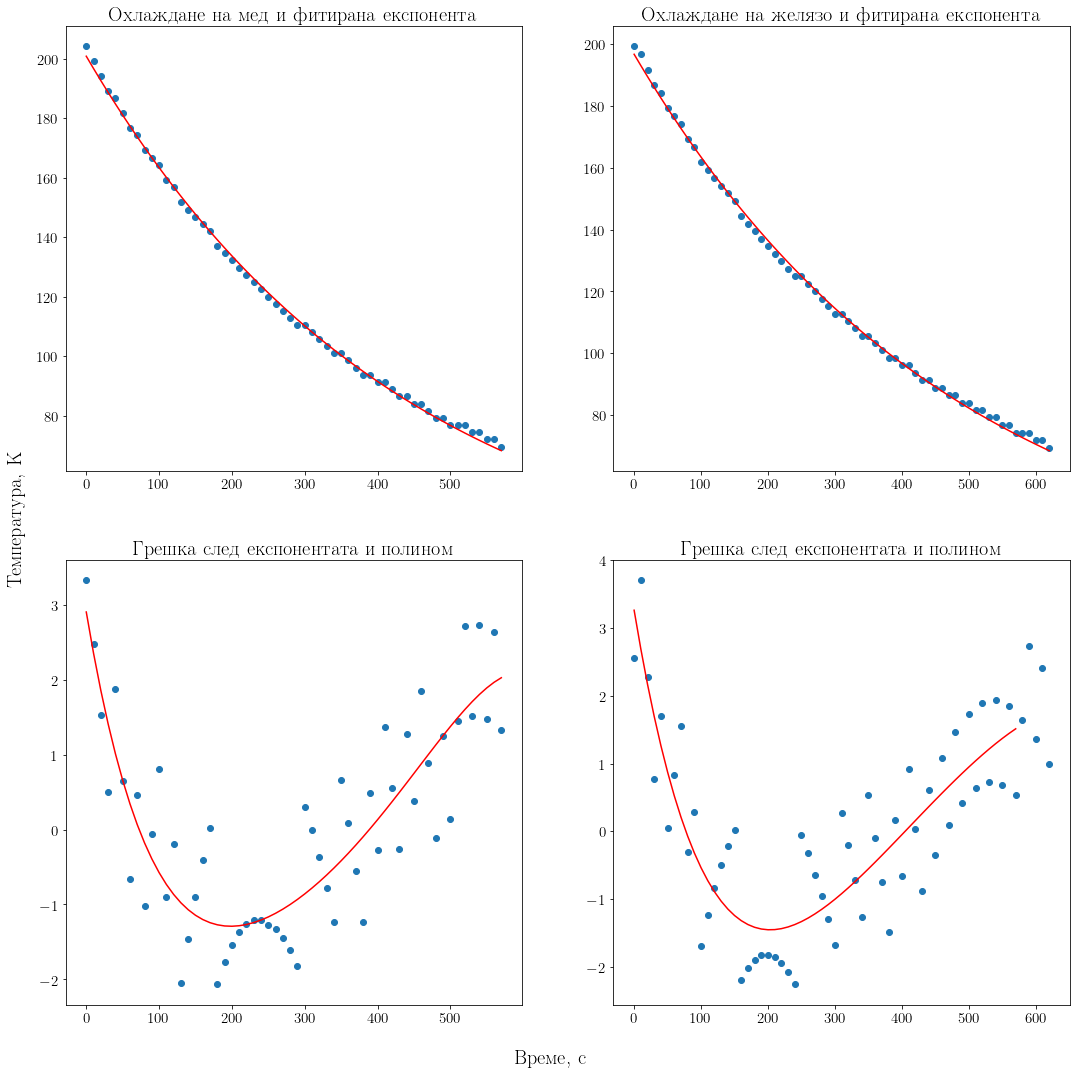
\includegraphics[width=0.9\columnwidth, keepaspectratio=true]{graph1.png}
\end{figure}

\end{document}